% ═══════════════════════════════════════════════════════════════════════════════
% CHAPTER 1 — PROJECT OVERVIEW
% End-of-Study Report — MES-X Dependency Traceability System
% ═══════════════════════════════════════════════════════════════════════════════

\chapter{Project Overview}
\label{chap:project-overview}

% ─────────────────────────────────────────────────────────────────────────────
\section{Introduction}
\label{sec:overview-intro}

This chapter establishes the professional and technical context of the
end-of-study internship project. It presents the host company, the industrial
environment in which the work was carried out, the problem that motivated the
project, and the main objectives assigned during the internship.

This context is important because the technical decisions described in the next
chapters were shaped by concrete industrial constraints: a large microservices
landscape, a growing number of Azure DevOps artifacts, and the operational need
for faster and more reliable traceability.

% ─────────────────────────────────────────────────────────────────────────────
\section{Host Company}
\label{sec:host-company}

\subsection{The Forvia Group}
\label{subsec:forvia-group}

Forvia is one of the world's leading automotive technology groups, formed
through the strategic merger of two major European industrial players:
\textbf{Faurecia}, a global specialist in automotive seating, interiors, and
emissions control technologies, and \textbf{HELLA}, a globally recognized
leader in automotive lighting systems and electronic components. The merger
created a group of exceptional scale, combining complementary technological
portfolios and international footprints to serve automotive manufacturers
across every major global market.

Forvia operates across more than 40 countries, employs over 150,000 people
worldwide, and maintains a strong research and development focus aimed at
accelerating the transition toward sustainable, intelligent, and connected
vehicles. Its product and technology portfolio spans seating systems, cockpit
electronics, clean mobility solutions, lighting, and sensors — placing the
group at the intersection of several of the most critical transformation
vectors in the modern automotive industry.

\subsection{Forvia Informatique Tunisie}
\label{subsec:forvia-tunisie}

The internship took place at \textbf{Forvia Informatique Tunisie}, the
Tunisian IT and digital engineering hub of the Forvia Group. Established as a
center of technical excellence within the group's global digital organization,
this entity is responsible for the design, development, and long-term
maintenance of the software systems that support industrial operations at
Forvia's manufacturing facilities worldwide.

Forvia Informatique Tunisie concentrates a multidisciplinary team of software
engineers, architects, DevOps specialists, and technical leads who work in close
collaboration with operational and product teams across multiple Forvia business
units. The entity contributes to a broad range of digital initiatives, including
manufacturing execution systems, production monitoring platforms, enterprise
integration solutions, and internal tooling designed to improve the efficiency
and traceability of the group's software delivery processes.

\subsection{The MES X.0 Division}
\label{subsec:mes-division}

The project was carried out within the \textbf{MES X.0} division of Forvia
Informatique Tunisie. This division is responsible for the design, development,
and evolution of a next-generation Manufacturing Execution System — a class of
industrial software that serves as the operational backbone of manufacturing
plants by orchestrating, monitoring, and recording all production activities
in real time.

The MES X.0 platform is built on a \textbf{microservices architecture}, a
deliberate technical choice that enables independent development, deployment,
and scaling of each functional domain of the system. Rather than a single
monolithic application, the platform is composed of dozens of specialized
services — each responsible for a specific manufacturing concern such as
production scheduling, quality control, equipment monitoring, or operator
guidance — that communicate through well-defined APIs and messaging contracts.

This architecture gives the platform exceptional flexibility and scalability:
new manufacturing capabilities can be added as new services, existing services
can be updated independently without impacting the whole system, and different
plants can be equipped with different subsets of the platform's services
according to their specific operational needs. The MES X.0 platform is deployed
and actively used at multiple Forvia manufacturing sites around the world,
processing real-time production data from industrial equipment and human
operators simultaneously.

However, this architectural flexibility comes with a corresponding increase in
the complexity of the software development process — a complexity that directly
motivated the project described in this report.

% ─────────────────────────────────────────────────────────────────────────────
\section{Project Context and Problem Statement}
\label{sec:project-context}

\subsection{Development Environment at Forvia}
\label{subsec:dev-environment}

At Forvia, \textbf{Azure DevOps} serves as the central platform for the
software development lifecycle across all digital teams. It provides an
integrated suite of tools covering the full range of development activities:
sprint and release planning through work item boards, source code management
through Git repositories, code review and integration through pull requests,
automated build and deployment pipelines through Azure Pipelines, and artifact
management for binaries and package versions.

Within the MES X.0 division specifically, Azure DevOps manages the development
activities of all microservices simultaneously. A given sprint may involve
planned work across ten, twenty, or more independent services, each progressing
at its own pace with its own team, its own repository, and its own release
cadence. The platform accumulates an ever-growing set of interconnected
artifacts: work items describing requirements and tasks, pull requests
integrating code changes, commits recording individual code modifications,
branches isolating development streams, and repository tags marking release
points.
\begin{figure}[H]
\centering
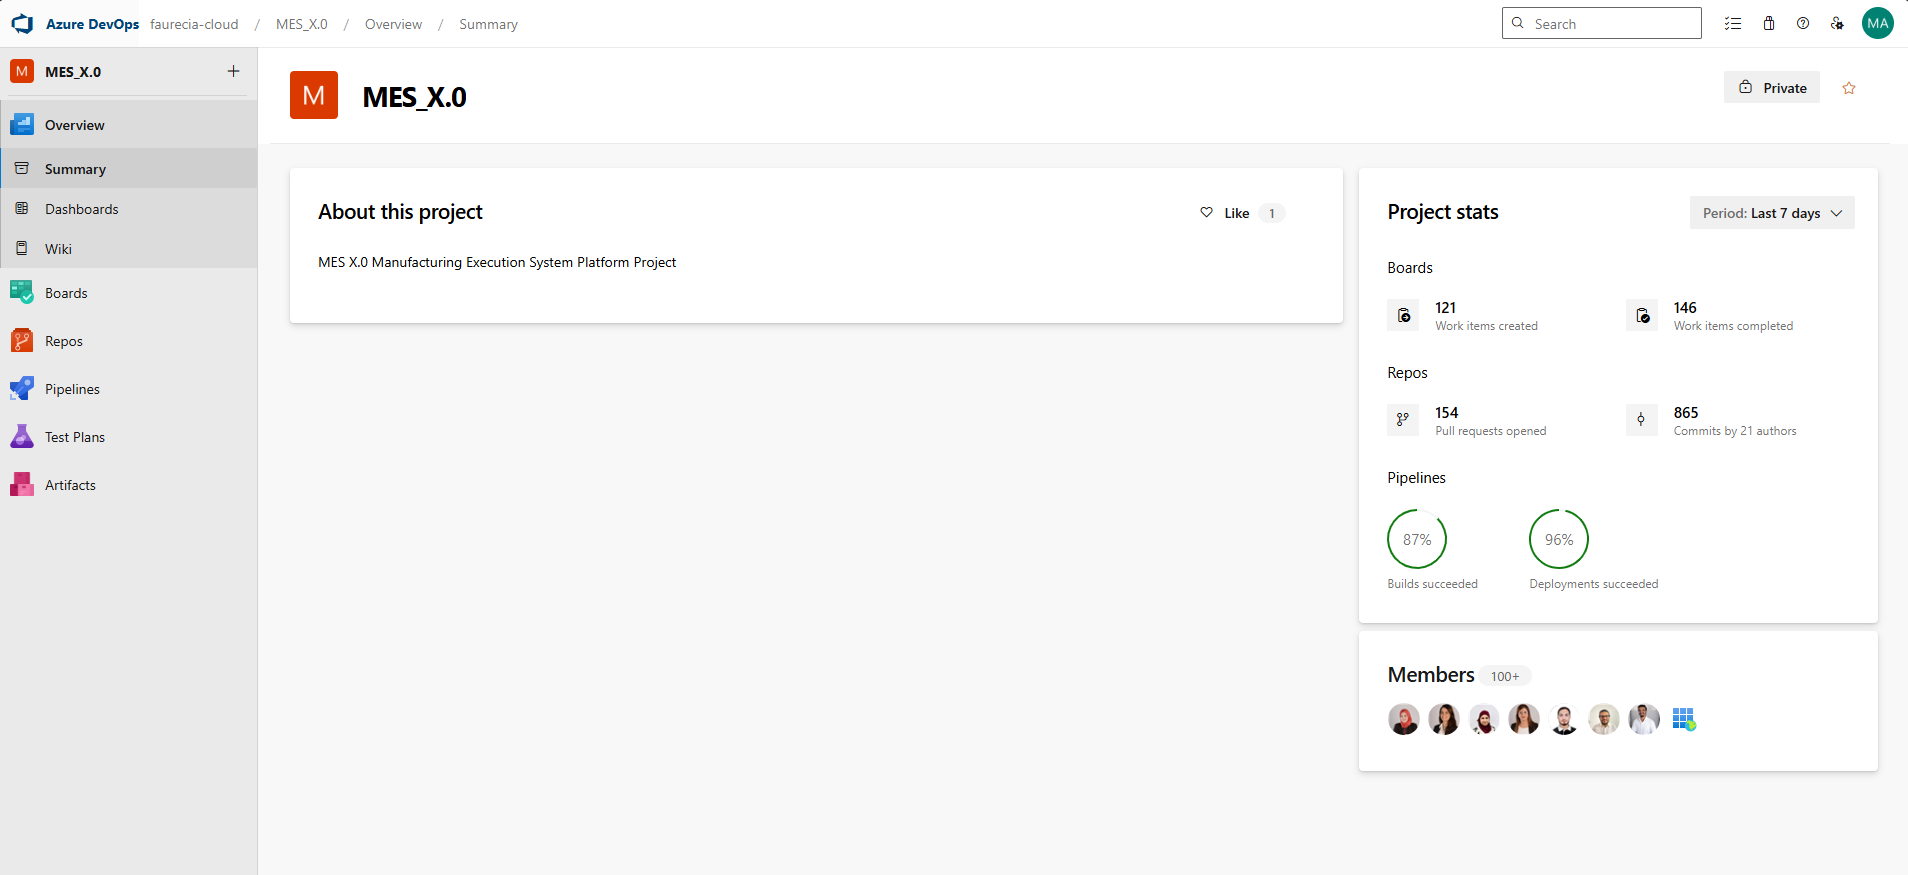
\includegraphics[width=0.95\linewidth]{img/overview/azure_board.png}
\caption{Azure DevOps environment used within the MES X.0 division, showing work item tracking and development workflow management}
\label{fig:azure-devops-board}
\end{figure}
\subsection{The Traceability Challenge}
\label{subsec:traceability-challenge}

In this multi-service, high-velocity development environment, a single
user-facing requirement — expressed as a work item at the Epic or Feature level
in Azure DevOps — typically decomposes into dozens of lower-level tasks, each
of which produces its own chain of development artifacts: a branch, one or more
commits, a pull request, and eventually a repository tag when the change is
released.

Understanding the complete impact of a requirement — or conversely, understanding
what requirements are affected by a change in a specific repository — requires
navigating this artifact chain in its entirety. For a release engineer
preparing a production deployment, this means answering questions such as:

\begin{itemize}
  \item Which work items are included in this release, and are they all in a
  completed state?
  \item For each work item, which pull requests carried the implementation, and
  in which repositories?
  \item For each repository, which commits were produced, and do they appear
  before or after the relevant release tag?
  \item Are there any commits that straddle a release boundary — present in one
  environment but not yet in another?
\end{itemize}

Before this project, answering these questions required a \textbf{manual and
entirely ad-hoc process}. The release engineer or developer would begin from a
work item in Azure DevOps, navigate to its linked pull requests, open each PR
to identify the target repository, navigate to the repository's commit history,
search for the relevant commits, check branch and tag references, and then
repeat the entire sequence for every related work item. Data extracted at each
step was typically recorded manually in spreadsheets to maintain a working
reference.

This process presented several critical limitations:

\begin{itemize}
  \item \textbf{Time cost}: a complete dependency trace for a single feature
  involving multiple services could require an entire working day to complete
  manually.
  \item \textbf{Error proneness}: the manual correlation of data across multiple
  Azure DevOps interfaces introduced a significant risk of missed links,
  incorrect associations, and incomplete coverage.
  \item \textbf{Non-reproducibility}: two engineers performing the same trace
  independently could arrive at different results depending on the path they
  followed and the data they chose to record.
  \item \textbf{Scalability failure}: as the number of microservices grew and
  development velocity increased, the manual approach became increasingly
  impractical, consuming disproportionate engineering time during critical
  release preparation phases.
\end{itemize}

\subsection{Project Motivation}
\label{subsec:motivation}

These limitations created a clear and urgent need for an automated solution.
The \textbf{MES-X Dependency Management} project was initiated within the
MES X.0 division to address this need directly: to design and implement a
system that would automate the reconstruction of dependency chains across Azure
DevOps artifacts, transforming a time-consuming and error-prone manual process
into a fast, reliable, and reproducible analytical capability.

The project was scoped as an end-of-study internship project, representing an
opportunity to deliver genuine industrial value while applying and extending
the software engineering knowledge acquired during the academic program.

% ─────────────────────────────────────────────────────────────────────────────
\section{Project Description}
\label{sec:project-description}

\subsection{Project Objectives}
\label{subsec:objectives}

The primary goal of the MES-X Dependency Management project is to design and
implement an \textbf{automated dependency traceability system} that replaces
the existing manual process with a reliable, efficient, and scalable solution
integrated into the Azure DevOps ecosystem.

The project pursues the following specific objectives:

\subsubsection{Automated Microservice Tag Identification}

The system must automatically identify and associate the relevant microservice
repository tags with work items by analyzing commit history and repository
metadata. This capability eliminates the need for manual navigation through
repository tag lists and commit histories, and ensures that the release context
of each code change is determined programmatically and consistently.

\subsubsection{Comprehensive Dependency Mapping}

The system must construct and expose complete traceability links across the full
chain of development artifacts: from high-level work items through pull requests
and commits down to repository branches and tags. This mapping must be complete
— covering all levels of the work item hierarchy and all artifact types — and
consistent across successive analysis sessions.

\subsubsection{Significant Reduction of Manual Effort}

By automating data retrieval, traversal, normalization, and aggregation, the
system must reduce the time required to perform a complete dependency analysis
from hours to seconds. This reduction must be sustained even for complex
analysis scenarios involving multiple work items and many repositories.

\subsubsection{Improved Data Accuracy and Consistency}

The system must eliminate the class of errors introduced by manual data
extraction and correlation. All dependency data must be derived from the same
authoritative source — the Azure DevOps APIs — through a standardized and
reproducible process, ensuring that results are accurate and identical across
successive runs for the same input.

\subsubsection{End-to-End Traceability}

The system must enable a user to trace any work item from its initial
description to the exact commits and microservice tags it affected, entirely
within a single analysis session. No cross-tool navigation or manual correlation
should be required to obtain a complete dependency view.

\subsubsection{Reusable and Scalable Architecture}

The system must be built on a modular, maintainable architecture that can be
extended to support additional artifact types, additional analysis modes, or
integration into other Forvia digital platforms — without requiring a
fundamental redesign of the existing system.

\subsection{Technical Scope}
\label{subsec:technical-scope}

The project encompasses the design and implementation of three interconnected
technical components: a backend service, a frontend application, and an
Azure DevOps integration layer.

\subsubsection{Backend Development}

The backend was developed using \textbf{NestJS} with TypeScript, a framework
chosen for its native support of modular architecture, dependency injection,
and TypeScript-first development — properties well-suited to the clean,
maintainable design required by this project.

The backend's responsibilities include:

\begin{itemize}
  \item Secure integration with the Azure DevOps REST APIs using Personal Access
  Token authentication.
  \item Normalization of raw Azure DevOps responses into structured, typed Data
  Transfer Objects that form the stable internal data model of the system.
  \item Recursive traversal of work item dependency graphs across multiple
  hierarchy levels and relation types.
  \item Resolution of pull requests, commits, repository branches, and Git tags
  for each node in the dependency graph.
  \item Implementation of batch processing strategies to minimize API call
  volume and respect rate limits.
  \item Implementation of Server-Sent Events streaming for progressive delivery
  of large analysis results.
  \item Exposure of well-documented RESTful endpoints, complemented by
  interactive Swagger documentation for developer exploration and testing.
\end{itemize}

\subsubsection{Frontend Application}

The frontend was developed using \textbf{Vue 3} with the Quasar framework,
providing a production-grade, responsive interface for initiating and exploring
dependency analyses. The frontend's role is not limited to presentation: it
actively participates in the orchestration of analysis sessions by managing
asynchronous backend calls, assembling view state from streamed results, and
providing real-time progress feedback to the user.

Key features of the frontend include:

\begin{itemize}
  \item Interactive visualization of work item dependency graphs, presenting
  hierarchical relationships, pull request links, and commit references in a
  structured and navigable form.
  \item Real-time batch processing interface powered by Server-Sent Events,
  allowing users to observe analysis progress incrementally rather than waiting
  for a single blocking response.
  \item Clear presentation of relationships between work items, pull requests,
  commits, branches, and tags, organized by repository and analysis mode.
  \item A dedicated Decision Dashboard that presents the release classification
  output of the aggregation component in an actionable, decision-ready format.
  \item A responsive and operationally focused design, tailored for everyday
  use by release engineers and development team leads.
\end{itemize}

\subsubsection{Azure DevOps Integration and Data Processing}

The solution relies on the Azure DevOps REST API as its exclusive data source.
The integration layer is responsible for all communication with this external
system and implements several mechanisms to ensure reliability and efficiency:

\begin{itemize}
  \item Authentication via Personal Access Tokens with secure credential
  management.
  \item Intelligent batching and concurrency control to respect Azure DevOps
  API rate limits during high-volume analysis sessions.
  \item A robust dependency resolution engine capable of recursive graph
  traversal, entity deduplication, and cross-module result normalization.
  \item Structured error handling and retry logic for transient API failures,
  ensuring that partial external failures do not silently corrupt analysis
  results.
\end{itemize}

\subsection{Project Activities}
\label{subsec:activities}

The project followed a structured development lifecycle organized around the
following phases:

\begin{itemize}
  \item \textbf{Requirements Analysis}: study of the existing manual
  traceability workflow, interviews with release engineers and developers, and
  formalization of the system's functional and non-functional requirements.

  \item \textbf{System Design and Architecture}: definition of the three-layer
  architecture, identification of the four main backend components, design of
  API contracts and data transfer objects, and preparation of the frontend
  structure.

  \item \textbf{Backend Implementation}: development of the Azure DevOps
  integration layer, recursive traversal logic, pull request resolution,
  commit and tag processing services, and progressive streaming support.

  \item \textbf{Frontend Development}: implementation of the main analysis
  views, centralized state management with Pinia, integration of real-time SSE
  updates, and development of the Decision Dashboard.

  \item \textbf{Testing and Validation}: unit testing of backend services and
  utilities, validation of backend contracts against frontend needs, and
  end-to-end checks for the main analysis scenarios.

  \item \textbf{Integration and Optimization}: performance tuning of graph
  traversal and batch resolution, implementation of in-memory caching, and
  verification of result consistency across analysis modes.

  \item \textbf{Deployment Preparation}: backend containerization with Docker,
  environment configuration, CI/CD pipeline setup, and completion of Swagger
  documentation for developer handoff.
\end{itemize}

% ─────────────────────────────────────────────────────────────────────────────
\section{Conclusion}
\label{sec:overview-conclusion}

This chapter has presented the industrial setting of the MES-X Dependency
Management project and clarified why dependency tracing had become a real
operational issue. In a large microservices ecosystem, manual analysis no
longer provides the speed, consistency, or reliability required for release
preparation.

The next chapter translates that problem into a formal requirements
specification. It defines what the system must deliver functionally and which
quality constraints it must satisfy in practice.